\documentclass[11pt]{article}
\usepackage{amsmath,textcomp,amssymb,geometry,graphicx,enumerate}

\def\Name{Vijay Hans}  % Your name
\def\SID{3041285081}  % Your student ID number
\def\PreLab{3} % Number of Homework
\def\Session{Spring 2026}
\def\Cls{PHYS 5BL}
\title{\Cls--Spring 2026 --- Pre-Lab \PreLab \ Response}
\author{\Name, SID \SID}
\markboth{\Cls -- \Session\  Pre-Lab \PreLab\ \Name}{\Cls -- \Session\ Pre-Lab \PreLab\ \Name}
\pagestyle{myheadings}
\date{\today}

\newenvironment{qparts}{\begin{enumerate}[{(}a{)}]}{\end{enumerate}}
\def\endproofmark{$\Box$}
\newenvironment{proof}{\par{\bf Proof}:}{\endproofmark\smallskip}

\textheight=9in
\textwidth=6.5in
\topmargin=-.75in
\oddsidemargin=0.25in
\evensidemargin=0.25in
\setlength{\parindent}{0pt}

\begin{document}
\maketitle

\begin{enumerate}
    \item 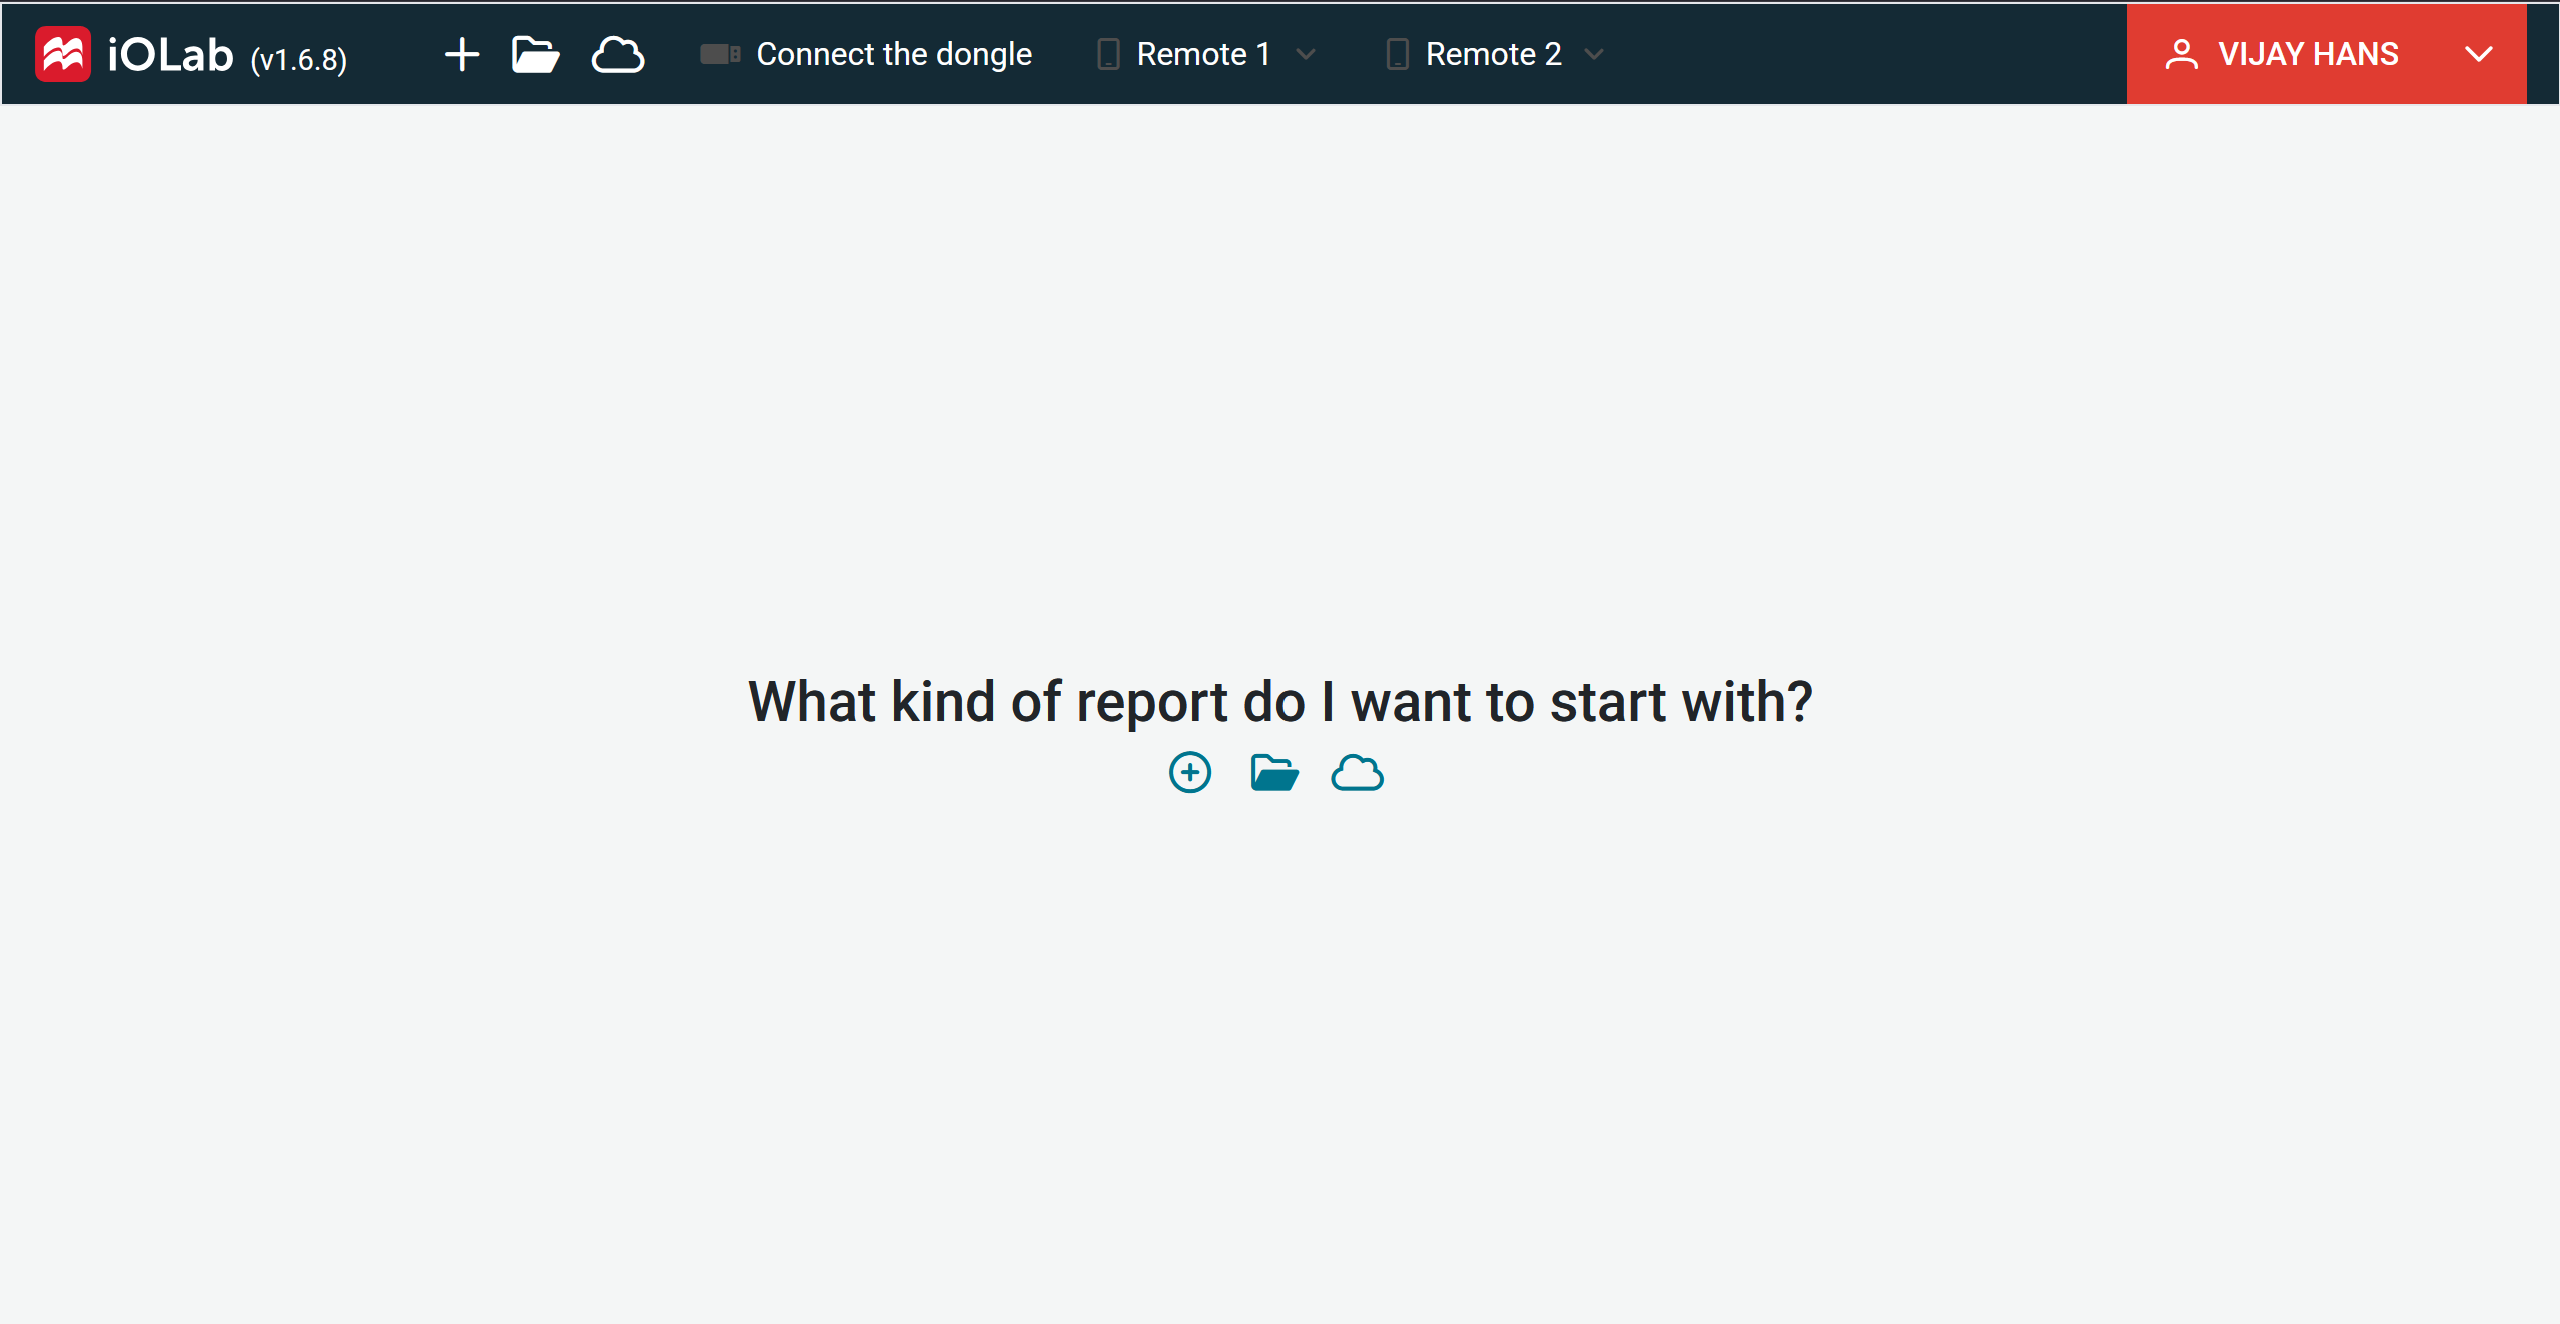
\includegraphics[scale=0.5]{iolabs confirmation.png}
    \item Averaging these estimates doesn't eliminate systematic bias. The crowd here has never seen Qin Shi Huang Di, so the population of guesses isn't necessarily centered on his actual height but rather on some "consensus guess" as to what his height is. The more estimates you take, the more you converge on a value which is not necessarily the Emperor's actual height. In other words, these estimates only tell us about what the people think about the emperor's height, and nothing about the emperor's height itself.
\end{enumerate}

\end{document}